\documentclass[twocolumn,10pt,a4paper]{article}
\usepackage[utf8]{inputenc}
\usepackage[T1]{fontenc}
\usepackage{geometry}
\geometry{top=20mm,bottom=25mm,left=15mm,right=15mm,columnsep=8mm}
\usepackage{amsmath,amssymb}
\usepackage{booktabs}
\usepackage{titlesec}
\usepackage[expansion=false]{microtype}
\usepackage{enumitem}
\usepackage{array}
\usepackage{graphicx}
\usepackage{tikz}
\usetikzlibrary{arrows.meta,positioning,fit,backgrounds,shapes.geometric,calc}
\usepackage{pgfplots}
\pgfplotsset{compat=1.18}
\usepackage{tcolorbox}
\tcbuselibrary{skins,breakable}
\usepackage{listings}
\usepackage{caption}
\usepackage[hidelinks,colorlinks=true,linkcolor=black,citecolor=black,urlcolor=black]{hyperref}

% ---------------------------------------------------------------------
% Grayscale palette
% ---------------------------------------------------------------------
\usepackage{xcolor}
\definecolor{mfdarkblue}{HTML}{111111}
\definecolor{mfblue}{HTML}{333333}
\definecolor{mfteal}{HTML}{444444}
\definecolor{mfamber}{HTML}{555555}
\definecolor{mfred}{HTML}{000000}
\definecolor{mfgrey}{HTML}{6B7280}
\definecolor{mflightgrey}{HTML}{F2F3F5}
\definecolor{mfcodebg}{HTML}{F7F7F9}
\definecolor{mfgreen}{HTML}{222222}

% ---------------------------------------------------------------------
% Section title formatting
% ---------------------------------------------------------------------
\titleformat{\section}
  {\normalfont\large\bfseries}
  {\thesection}{1em}{}
\titleformat{\subsection}
  {\normalfont\normalsize\bfseries}
  {\thesubsection}{1em}{}
\titleformat{\subsubsection}
  {\normalfont\normalsize\bfseries\itshape}
  {\thesubsubsection}{1em}{}

% List spacing
\setlist[enumerate]{topsep=2pt, itemsep=2pt, parsep=2pt}
\setlist[itemize]{topsep=2pt, itemsep=2pt, parsep=2pt}

% ---------------------------------------------------------------------
% Code listing style
% ---------------------------------------------------------------------
\lstdefinestyle{code}{
  backgroundcolor=\color{mfcodebg},
  basicstyle=\ttfamily\footnotesize,
  keywordstyle=\color{mfdarkblue}\bfseries,
  commentstyle=\color{mfgrey}\itshape,
  stringstyle=\color{mfteal},
  numbers=left,
  numberstyle=\tiny\color{mfgrey},
  numbersep=8pt,
  frame=single,
  framerule=0.4pt,
  rulecolor=\color{mfgrey!60},
  breaklines=true,
  breakatwhitespace=false,
  showstringspaces=false,
  tabsize=2,
  xleftmargin=1em,
  xrightmargin=0.2em,
  aboveskip=8pt,
  belowskip=8pt,
  columns=fullflexible,
  keepspaces=true,
}
\lstset{style=code}
\lstdefinelanguage{asl}{
  morekeywords={if,else,for,not},
  sensitive=false,
  morecomment=[l]{//},
  morestring=[b]",
}

% ---------------------------------------------------------------------
% Callout boxes (grayscale)
% ---------------------------------------------------------------------

\newtcolorbox{notebox}[1][]{
  breakable, enhanced,
  colback=black!4, colframe=black!65,
  coltitle=white, colbacktitle=black!65,
  fonttitle=\bfseries,
  title={NOTE},
  boxrule=0.6pt, arc=1.5pt, outer arc=1.5pt,
  left=6pt,right=6pt,top=4pt,bottom=4pt,
  #1
}
\newtcolorbox{strengthbox}[1][]{
  breakable, enhanced,
  colback=black!3, colframe=black!50,
  coltitle=white, colbacktitle=black!50,
  fonttitle=\bfseries,
  title={DESIGN NOTE},
  boxrule=0.6pt, arc=1.5pt, outer arc=1.5pt,
  left=6pt,right=6pt,top=4pt,bottom=4pt,
  #1
}

\newcommand{\code}[1]{\texttt{\small #1}}
\newcommand{\file}[1]{\texttt{#1}}

% ---------------------------------------------------------------------
% Title block
% ---------------------------------------------------------------------
\title{\vspace{-10mm}\textbf{\Large Matrix\_Factory: A Holonic Hydrogen-Plant Digital Twin --- Architecture, Multi-Agent Coordination, and Physical Simulation}}
\author{
  \textbf{Technical Report} \\
  \small Matrix\_Factory Digital Twin Project \\ \vspace{1mm}
  \small Stack: Python 3 physical engine (Numba/Cython, CoolProp) $\leftrightarrow$ gRPC $\leftrightarrow$ Java 17 / JaCaMo \\
  \small (Jason + CArtAgO + MoISE) $\leftrightarrow$ WebSocket $\leftrightarrow$ browser dashboard
}
\date{\small \today}

\begin{document}

\maketitle


\vspace{2mm}
\tableofcontents
\vspace{2mm}

% =======================================================================
\section*{Executive Summary}
\addcontentsline{toc}{section}{Executive Summary}

Matrix\_Factory is a co-simulation testbed that couples a numerically detailed hydrogen-technology physics engine with a cognitive, holonic multi-agent factory-control layer, wired together through a lock-stepped gRPC time-synchronisation protocol and exposed to the outside world through an authenticated WebSocket telemetry feed and a canvas-based live dashboard. The system compares two competing shop-floor control philosophies --- \textbf{PROSA} (heterarchical, peer-negotiated) and \textbf{ADACOR} (hierarchical, supervisor-directed) --- under a simulated disturbance (an electricity-price spike), using a production-quality-coupled hydrogen fuel-cell test bench as the fifth station in a five-stage manufacturing line.

This report details the implementation of Matrix\_Factory, focusing on the system architecture, multi-agent coordination, and physical simulation engine. The architecture spans multiple languages and paradigms, integrating continuous-time numerical models in Python with discrete event-driven agent reasoning in Java (Jason \code{.asl} and MoISE XML). The following sections outline the technical foundation, including the communication bridge, the agent negotiation protocols, and the physical models.

\textbf{Key System Capabilities:}
\begin{itemize}
\item A physically grounded PEMFC electrochemical model (Nernst potential, activation/ohmic/concentration overpotentials, Newton--Raphson inversion) with a JIT-compiled, thread-isolated batch polarisation sweep and a documented, single-source-of-truth failure-flag bitmask.
\item A carefully argued distributed-systems core: a two-phase-commit protocol for live organisational-schema transitions (PROSA~$\leftrightarrow$~ADACOR), a Contract-Net negotiation protocol with an atomic, race-free resource/AMR reservation path, and a cooperative space-time A* fleet router.
\item Detailed in-source documentation of concurrency handling and distributed-systems challenges directly within the \code{.asl} and \code{.java} implementations.
\item A secure, purpose-built telemetry channel (HMAC-signed, short-lived WebSocket tickets) and a horizontally-scaled experiment harness that mechanically clones the entire agent society 30$\times$ into one JVM via source-level token rewriting.
\end{itemize}

Early development phases addressed several integration challenges, including unit conversion consistency, dead code elimination, and time-synchronisation wiring. The current system represents a stable, fully functional state capable of producing valid empirical data for the central experiment.

% =======================================================================
\section{Introduction}

This report describes the architecture and implementation of the \textbf{Matrix\_Factory} system. The document outlines the subsystems that make up the digital twin, including the physical simulation engine, the multi-agent cognitive layer, the integration middleware, and the telemetry dashboard. The presentation is structured bottom-up, detailing the design decisions and technical implementations across the Python, Java, and Jason components.

\subsection{What the project is}
Matrix\_Factory is a \textbf{digital twin of a small hydrogen-technology manufacturing line}: five stations producing and end-of-line-testing PEM fuel-cell stacks, served by a two-vehicle AMR (autonomous mobile robot) fleet, and controlled by a society of BDI (belief-desire-intention) agents implementing two competing organisational philosophies from the manufacturing-systems literature:

\begin{itemize}
\item \textbf{PROSA} (Product-Resource-Order-Staff Architecture) --- a heterarchical, holonic model in which order holons and resource holons negotiate as peers via a Contract-Net Protocol (CNP), with no built-in authority hierarchy.
\item \textbf{ADACOR} (ADAptive holonic COntrol aRchitecture) --- a hierarchical variant in which a supervisor holon can assert direct authority over resource and order holons, intended for use under disturbance conditions where centralised re-coordination is faster than renegotiation.
\end{itemize}

The motivating research question is whether switching from PROSA to ADACOR during an energy-price spike measurably improves throughput, tardiness, or work-in-process compared to remaining in PROSA throughout (\S\ref{sec:experiment}).

Stations 1--4 are stochastic black boxes (Gaussian processing time, Bernoulli defect roll). Station 5 is materially different: it is a genuine test bench backed by a numerically solved PEM fuel-cell electrochemical model running in a separate Python process, connected over gRPC, and it is causally coupled to the upstream stations through a purpose-built "manufacturing-quality bridge" (\S\ref{sec:quality-bridge}) that turns Stations 1--4's logged defects and processing-time variance into physical derating parameters (added ohmic resistance, reduced reactant activity) for the Station 5 polarisation sweep.

\subsection{Repository layout at a glance}
\begin{table*}[t]
\centering
\small
\begin{tabular}{@{}p{3.0cm}p{13.5cm}@{}}
\toprule
\textbf{Path} & \textbf{Contents} \\
\midrule
\file{physical\_engine/} & Python physics: PEMFC electrochemistry, stack thermal model, H\textsubscript{2} tank, compressor, station stochastics, CoolProp-backed lookup tables, Numba/Cython compute kernels, the gRPC \code{SimBridge} server. \\
\file{src/agt/} & Jason \code{.asl} agent programs: \code{supervisor\_agent}, \code{order\_holon}, \code{resource\_holon}, \code{amr\_agent}. \\
\file{src/org/} & MoISE organisational specifications: \code{prosa\_org.xml}, \code{adacor\_org.xml}. \\
\file{.../java/factory/} & CArtAgO artifacts and the Java-side simulation kernel (\code{MainSimulator}, \code{GrpcClientBridge}, station/AMR/telemetry/database artifacts). \\
\file{.../test/java/} & JUnit 5 invariant, seeded-replay, and system-integration tests. \\
\file{physical\_engine/\allowbreak factory\_simulation/\allowbreak *\_test.py} & Pytest physics unit tests. \\
\file{factory.jcm} & The JaCaMo topology: agents, artifacts, workspaces, organisations, for a single run. \\
\file{scripts/}, \file{experiments/}, \file{analysis/} & Phase-4 mega-topology generation, the PROSA-vs-ADACOR experiment driver, and its Monte Carlo replication results (\S\ref{sec:experiment}). \\
\file{visualization/} & Canvas-based live dashboard (\file{dashboard.js}, \file{index.html}, \file{factory\_layout.json}). \\
\file{docs/} & Design documents and phase-by-phase development history (treated as background only in this report). \\
\bottomrule
\end{tabular}
\end{table*}

% =======================================================================
\section{System Architecture}
\label{ch:architecture}

\subsection{Three-tier co-simulation}
The system is composed of three processes cooperating under a hard time-synchronisation contract, plus one passive observer (Figure~\ref{fig:architecture}):

\begin{enumerate}
\item \textbf{The physical federate} (Python, \file{physical\_engine/sim\_bridge\_server.py}) --- owns all continuous physical state (stack voltage, temperature, tank pressure, compressor power) and exposes it over gRPC.
\item \textbf{The cognitive/orchestration federate} (Java 17, JaCaMo: Jason + CArtAgO + MoISE, \file{src/main/java/factory/}, \file{src/agt/}, \file{src/org/}) --- owns discrete event logic: order lifecycle, negotiation, transport, and organisational-schema transitions. \code{MainSimulator} plays the role of \emph{Time Management Coordinator} (TMC) in an HLA-like (High Level Architecture) co-simulation pattern.
\item \textbf{The telemetry/visualisation tier} (embedded Tyrus WebSocket server + static JS/canvas dashboard) --- a read-only observer fed by the TMC once per tick.
\end{enumerate}

\begin{figure*}[t]
\centering
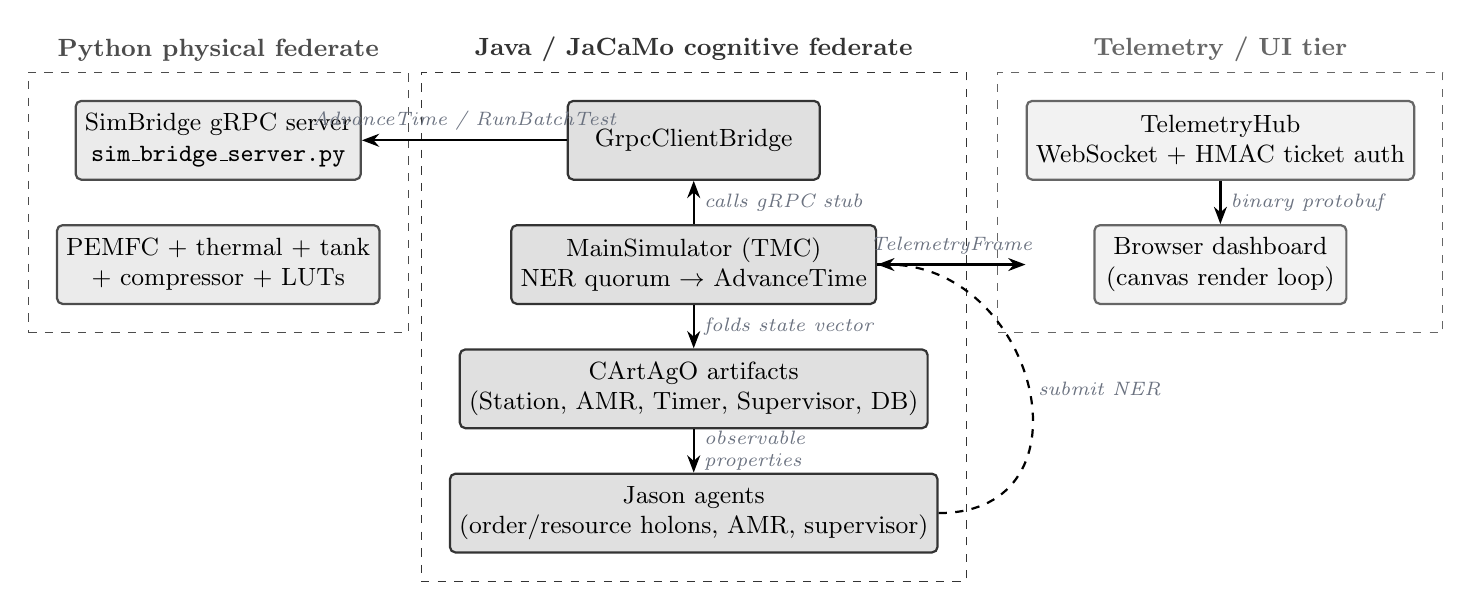
\begin{tikzpicture}[
  box/.style={draw, rounded corners=2pt, minimum width=3.2cm, minimum height=1.0cm, align=center, font=\small, line width=0.8pt},
  pybox/.style={box, fill=black!8, draw=black!70},
  javabox/.style={box, fill=black!12, draw=black!80},
  webbox/.style={box, fill=black!5, draw=black!60},
  lbl/.style={font=\scriptsize\itshape, color=mfgrey},
  arr/.style={-{Stealth[length=2.2mm]}, line width=0.8pt},
  darr/.style={arr, dashed}
]

% Python tier
\node[pybox] (sim) {SimBridge gRPC server\\\texttt{sim\_bridge\_server.py}};
\node[pybox, below=0.55cm of sim] (physics) {PEMFC + thermal + tank\\+ compressor + LUTs};
\node[fit=(sim)(physics), draw=black!70, dashed, inner sep=10pt, label={[black!70,font=\bfseries\small]above:Python physical federate}] (pytier) {};

% Java tier
\node[javabox, right=2.6cm of sim] (bridge) {GrpcClientBridge};
\node[javabox, below=0.55cm of bridge] (tmc) {MainSimulator (TMC)\\NER quorum $\rightarrow$ AdvanceTime};
\node[javabox, below=0.55cm of tmc] (cartago) {CArtAgO artifacts\\(Station, AMR, Timer, Supervisor, DB)};
\node[javabox, below=0.55cm of cartago] (jason) {Jason agents\\(order/resource holons, AMR, supervisor)};
\node[fit=(bridge)(tmc)(cartago)(jason), draw=black!80, dashed, inner sep=10pt, label={[black!80,font=\bfseries\small]above:Java / JaCaMo cognitive federate}] (javatier) {};

% Web tier
\node[webbox, right=2.6cm of bridge] (ws) {TelemetryHub\\WebSocket + HMAC ticket auth};
\node[webbox, below=0.55cm of ws] (dash) {Browser dashboard\\(canvas render loop)};
\node[fit=(ws)(dash), draw=black!60, dashed, inner sep=10pt, label={[black!60,font=\bfseries\small]above:Telemetry / UI tier}] (webtierbox) {};

% Cross-tier arrows
\draw[arr] (bridge.west) -- node[lbl,above]{AdvanceTime / RunBatchTest} (sim.east);
\draw[arr] (tmc.east) -- node[lbl,above]{TelemetryFrame} (ws.west |- tmc.east);
\draw[arr] (ws.south) -- node[lbl,right]{binary protobuf} (dash.north);

% Java-tier internal flow arrows
\draw[arr] (tmc) -- node[lbl,right]{calls gRPC stub} (bridge);
\draw[arr] (tmc) -- node[lbl,right]{folds state vector} (cartago);
\draw[arr] (cartago) -- node[lbl,right,align=left]{observable\\properties} (jason);
\draw[darr] (jason.east) to[out=0,in=0,looseness=1.6] node[lbl,right]{submit NER} (tmc.east);

\end{tikzpicture}
\caption{Process topology. Time flows left to right on every tick: the TMC computes a bounded $dt$ from outstanding NextEventRequests (NER), calls \code{AdvanceTime} on the Python federate, folds the returned state vector into CArtAgO observable properties, and broadcasts a serialized \code{TelemetryFrame} to the WebSocket hub.}
\label{fig:architecture}
\end{figure*}

\subsection{The time-synchronisation contract}
\label{sec:time-sync}
The design vocabulary here is explicitly borrowed from HLA-style federated simulation:

\begin{itemize}
\item \textbf{NER (NextEventRequest):} a Jason agent about to block on a physical delay (station processing, transport) tells the TMC the simulation time at which it next needs to be woken, via \code{MainSimulator.submitNER(agentId, requestedNextTime)}.
\item \textbf{TMC (Time Management Coordinator):} \code{MainSimulator}'s tick loop (\file{MainSimulator.java}) waits on a \code{CountDownLatch} sized to the registered-agent count (13 in the single-run topology: 5 order holons + 5 stations + 2 AMRs + 1 supervisor), with a 10\,ms quorum timeout. It then computes $dt$ as the \emph{minimum} outstanding NER gap, clamped to $[\text{MIN\_DT}=0.01\text{s}, \text{MAX\_DT}=1.0\text{s}]$, and calls the physical federate's \code{AdvanceTime}.
\item \textbf{TAG (TimeAdvanceGrant):} conceptually, the signal that lets a waiting agent proceed once its requested time has been reached.
\end{itemize}

This is a legitimate and fairly sophisticated design for keeping the discrete agent layer and the continuous physical layer numerically consistent without simply free-running both on wall-clock time; the \emph{implementation} of the TAG side of this contract is realised procedurally, through agent polling of artifact-observable properties, rather than as an explicit callback or interrupt from the TMC back to a waiting agent.

\subsection{Organisational duality: PROSA and ADACOR co-resident}
\label{sec:org-duality}
Both MoISE organisational specifications are loaded \emph{simultaneously} for the full agent roster in \file{factory.jcm} --- every agent is declared as a player of both \code{factory\_prosa\_org} and \code{factory\_adacor\_org} from the moment the topology boots (see Listing~\ref{lst:jcm-orgs}). There is no runtime "switch the loaded organisation" operation; instead, a Jason belief \code{active\_schema(prosa|adacor)} in \code{supervisor\_agent.asl}, together with an integer \code{schema\_epoch} threaded through the gRPC \code{TimeStep}/\code{TelemetryFrame} messages, gates which behavioural branches fire. The actual reconfiguration event is a bespoke two-phase-commit protocol (\S\ref{sec:2pc}) rather than a MoISE-level group/scheme reformation. The authority link declared in \code{adacor\_org.xml} (\code{supervisor}~$\to$~\code{resource\_holon}) is therefore not structurally enforced by the MoISE middleware at runtime; rather, it is a design-level constraint that the Jason plans approximate procedurally.

\begin{figure*}[t]
\begin{lstlisting}[language=,caption={Both organisations are populated with the identical, full agent roster at boot (\file{factory.jcm}).},label={lst:jcm-orgs}]
organisation factory_prosa_org : prosa_org.xml {
    group holonic_factory : shop_floor {
        players: supervisor supervisor, order_1 order_holon, ...
                 station_1 resource_holon, ..., amr_1 transport_holon, ...
    }
}
organisation factory_adacor_org : adacor_org.xml {
    group adaptive_factory : shop_floor {
        players: supervisor supervisor, order_1 order_holon, ...   // identical roster
    }
}
\end{lstlisting}
\end{figure*}

% =======================================================================
\section{The Physical Simulation Engine}
\label{ch:physics}

\subsection{Overview}
The Python package \file{physical\_engine/} implements the continuous-time physics behind Station 5 (the fuel-cell test bench) and its supporting utilities (hydrogen storage, compression). It is organised as:

\begin{table*}[t]
\centering
\small
\begin{tabular}{@{}p{3.6cm}p{12.9cm}@{}}
\toprule
\textbf{Module} & \textbf{Role} \\
\midrule
\file{core/} & Minimal shared types: \code{Component} base class, \code{TankState} enum, \code{StandardConditions}/\code{GasConstants}, \code{ComponentInitializationError}. \\
\file{factory\_simulation/\allowbreak pemfc\_model.py} & Nernst potential, activation/ohmic/concentration overpotentials, Newton--Raphson current-density solver, parallel batch polarisation sweep, failure-flag bitmask. \\
\file{factory\_simulation/\allowbreak stack\_thermal\_model.py} & Two-node (core/skin) lumped thermal capacitance model with coolant coupling. \\
\file{factory\_simulation/\allowbreak h2\_tank.py} & Two-tier (ideal-gas / real-gas LUT-inverted) hydrogen storage tank. \\
\file{factory\_simulation/\allowbreak compressor.py} & Single-stage polytropic compressor work. \\
\file{factory\_simulation/\allowbreak station\_stochastics.py} & Deterministic per-station RNG seeding + Gaussian processing time / Bernoulli defect helpers (mirrors the Java-side \code{BaseStationArtifact} logic for Python-side tests). \\
\file{optimization/\allowbreak lut\_manager.py} & CoolProp-backed pressure/temperature property lookup tables with bilinear interpolation, JIT batch lookup, and a bisection-based density$\to$pressure inversion. \\
\file{optimization/\allowbreak numba\_ops.py} & Public shim over a compiled Cython core (\file{\_numba\_ops\_core.pyx}) with a pure-Python fallback, gated by \code{H2PLANT\_HARDENED}. \\
\file{sim\_bridge\_server.py} & The gRPC \code{SimBridge} servicer: \code{AdvanceTime}, \code{RunBatchTest}, \code{HealthCheck}. \\
\bottomrule
\end{tabular}
\end{table*}

\subsection{PEMFC electrochemical model}
\label{sec:pemfc}
\file{pemfc\_model.py} implements a single-cell PEM fuel-cell voltage model in the \emph{subtractive} (fuel-cell, not electrolyzer) convention:
\[
V_{\text{stack}}(j) = N_{\text{cells}} \times \big(E_{\text{ocv}} - \eta_{\text{act}} - \eta_{\text{ohm}} - \eta_{\text{conc}}\big)
\]
with the open-circuit (Nernst) potential
\[
E_{\text{ocv}} = 1.229 - 0.85\times10^{-3}(T-298.15) + \frac{RT}{2F}\ln\!\big(a_{H_2}\, a_{O_2}^{0.5}\big),
\]
activation overpotential $\eta_{\text{act}} = \dfrac{RT}{\alpha z F}\ln(j/j_0)$ with $\alpha=0.5$, $z=4$ (the four-electron ORR pathway), $j_0 = 10^{-9}\,\text{A/cm}^2$; ohmic overpotential $\eta_{\text{ohm}} = j \cdot R_{\text{internal}}$; and a concentration overpotential $\eta_{\text{conc}} = -B\ln(1-j/j_{\text{lim}})$ with an explicit $C^1$-continuous linear extrapolation for $j/j_{\text{lim}} > 0.99$ so the sweep never hits the logarithmic singularity at $j_{\text{lim}}$.

\begin{strengthbox}
The module enforces its own physical-parameter isolation: a module-level runtime guard (\code{if PEMFCConstants.z\_pemfc != 4: raise RuntimeError(...)}) exists specifically so that the four-electron ORR kinetic constants used here can never be silently contaminated by the two-electron OER/HER constants from a legacy, structurally similar electrolyzer model referenced in the module's own docstring (\file{components/electrolysis/pem\_electrolyzer.py}, which is not present in this checkout). It also survives \code{python -O}, since the guard is a plain \code{if/raise} rather than an \code{assert}.
\end{strengthbox}

Given a target voltage, \code{newton\_raphson\_solver} inverts the curve for current density using an \emph{analytic} Jacobian (not finite differences) with a bracket-clamped Newton step, $\text{tol}=10^{-4}\,\text{V}$, and a 50-iteration cap. \code{batch\_polarization\_sweep} vectorises the forward curve over a 12-point (default) or caller-specified current-density sweep using \code{numba.prange}, with a pre-allocated per-thread scratchpad indexed by \code{i \% numba\_threads} --- the code comments explicitly note this is a deliberate substitute for \code{get\_thread\_id()}, which the surrounding documentation records as unreliable in this Numba configuration.

\subsubsection{Failure-flag bitmask}
A single \code{uint32} bitmask, defined once in \code{pemfc\_model.py} and imported everywhere else it is needed (explicitly to keep the flag values and the physics that set them from drifting apart), reports up to five independent failure modes:

\begin{table*}[t]
\centering
\small
\begin{tabular}{@{}cp{3.4cm}p{11.0cm}@{}}
\toprule
\textbf{Bit} & \textbf{Flag} & \textbf{Trigger} \\
\midrule
0 & \code{OHMIC\_DEGRADATION} & $\eta_{\text{ohm}}$ exceeds 0.35\,V at any swept point (membrane/contact resistance too high). \\
1 & \code{MASS\_TRANSPORT\_STARV} & Set by \file{sim\_bridge\_server.py}, not the physics kernel: measured voltage \emph{increases} between adjacent, increasing current-density points (a monotonicity violation). \\
2 & \code{THERMAL\_SHUTDOWN} & Requested test temperature exceeds 358.15\,K ($\sim$85\,\textdegree C). \\
3 & \code{LOW\_ACTIVATION} & $a_{H_2}$ or $a_{O_2}$ below 0.7 --- a reachable \emph{proxy} for catalyst degradation, since the model has no direct per-stack catalyst-health parameter. \\
4 & \code{SOLVER\_DID\_NOT\_CONV} & Reused, per an explicit code comment, as a general "comms failure / RPC error" flag on the Java side as well as a genuine non-convergence flag on the Python side. \\
\bottomrule
\end{tabular}
\end{table*}

\subsection{Manufacturing-quality bridge}
\label{sec:quality-bridge}
The manufacturing-quality bridge provides a causal link between discrete upstream events and continuous downstream physics. Stations 1--4 are otherwise context-free stochastic stations, but every \code{processOrder} call on \code{BaseStationArtifact} logs its Gaussian processing-time draw and Bernoulli defect roll to \code{DatabaseArtifact.recordStationQuality}, which accumulates an in-memory, per-stack \code{QualityProfile(defectCount, stationsVisited, cumulativeVarianceRatio)} in a Caffeine cache (bounded, 30-minute TTL to reclaim orphans from aborted stacks). When the stack reaches Station 5, \code{TestBenchArtifact.processOrder} performs a \emph{consuming read} of that profile (\code{qualityProfilesCache.asMap().remove(stackId)}) and converts it into two physical penalties carried on the gRPC \code{BatchTestRequest}:

\begin{equation*}
{\small R_{\text{int, eff}} = R_{\text{int}} + 0.08 \cdot \text{defectCount} + 0.02 \cdot \text{cumVarRatio}}
\end{equation*}
\[
\text{activity\_derate} = \min(0.6,\; 0.15 \times \text{defectCount})
\]

so that a poorly assembled stack shows up on the polarisation sweep as a genuinely steeper ohmic slope, and/or a reactant-starved (low-activation) curve, rather than as an artificial pass/fail coin flip layered on top of the physics. This end-to-end causal chain --- from upstream discrete-event manufacturing outcomes to downstream continuous electrochemistry --- is central to the system's claim of physical fidelity.

\subsection{Stack thermal model}
\code{StackThermalModel} is a two-node lumped-capacitance model (core temperature $T_{\text{core}}$, skin temperature $T_{\text{skin}}$) with heat generation from the electrochemical overpotentials ($Q_{\text{gen}} = I \times (\eta_{\text{act}} + \eta_{\text{ohm}})$, plus, in \file{sim\_bridge\_server.py}, an explicit standby heater term that clamps the stack to 353.15\,K/80\textdegree C when cold) and heat rejection to a coolant boundary condition at $T_{\text{coolant}}$. Validation tests (\file{test\_stack\_thermal.py}) check literature-style ordering ($T_{\text{core}} > T_{\text{skin}} > T_{\text{coolant}}$), steady-state convergence, decay behaviour, and energy conservation.


\begin{notebox}
$T_{\text{coolant}}$ is read from \code{ThermoStateIndex.CHILLER\_TEMP\_K} in the shared state vector. In the currently wired pipeline, this value is a boot-time constant (298.15\,K). 
\end{notebox}

\subsection{Hydrogen tank and compressor}
\code{TankArray} (\file{h2\_tank.py}) models a single 5\,kg-capacity, 0.5\,m$^3$ reservoir with a two-tier pressure model: an ideal-gas fallback ($p = \rho R_{H_2} T$) and, once the LUT manager is warm, a real-gas density-inversion lookup via CoolProp-backed tables (\S\ref{sec:lut}). \code{fill()} and \code{discharge()} are both capacity-clamped and lock-protected. \code{CompressorStage} (\file{compressor.py}) computes single-stage polytropic compression work from the shared \code{calculate\_compression\_work} JIT kernel, i.e.\ $W = \frac{\gamma}{\gamma-1}\cdot\frac{mRT_1}{\eta}\left[(P_2/P_1)^{x}-1\right]$.

\subsection{Lookup-table manager and real-gas properties}
\label{sec:lut}
\code{LUTManager} (\file{optimization/lut\_manager.py}, 1211 lines) pre-computes 2-D $(P,T)$ CoolProp property tables per fluid/property pair (density, enthalpy, entropy, and an $H(P,S)$ table for isentropic compressor work), then serves them via Numba-JIT bilinear interpolation with a documented, deliberate hybrid strategy: fast-path lookups inside the tabulated bounds, transparent fallback to a direct CoolProp call (with a warning log) outside them. \code{lookup\_pressure\_from\_density} inverts the $(P,T)\to D$ table by bisection (30 iterations, $10^{-4}$ relative tolerance) --- needed because CoolProp/the forward table only exposes $D(P,T)$, while \code{TankArray} needs the physically natural query "what pressure gives this density at this temperature."

\subsection{Numba/Cython dual compute core}
\file{optimization/numba\_ops.py} is a thin, well-designed shim: it prefers a compiled Cython extension (\code{\_numba\_ops\_core}), falls back to a pure-Python/Numba implementation (\code{\_numba\_ops\_core\_python.py}) for development, and --- if \code{H2PLANT\_HARDENED=1} is set --- refuses to fall back at all, raising \code{ImportError} immediately so a missing compiled artefact in a "hardened" deployment is loud rather than silently slow. The CI workflow (\S\ref{sec:ci}) actually exercises both configurations via a build matrix.

The shim's exported surface (\code{\_\_all\_\_}) is large: boiler flash/outlet-enthalpy solvers, a deoxo multi-zone PFR step, cyclone mechanics, a SOEC (solid-oxide electrolyzer) step, dry-cooler and interchanger flash solvers, Rachford--Rice and UV-flash routines, and more, alongside the handful of functions actually used here (bilinear interpolation, compression work, mixture enthalpy). This is consistent with \code{numba\_ops} being a shared compute core built for --- and by implication once serving --- a substantially larger plant simulation than the one wired up in this repository; the unused surface is otherwise inert and does not affect the Station 5 pipeline exercised in this report.

\subsection{Station-parameter reference}
\label{sec:stationdrift}
\file{factory\_simulation/station\_stochastics.py} defines \code{STATION\_PARAMS}, a dictionary of reference processing parameters for Stations 1--4. These constants serve as validation references for the physical engine, while the actual stochastic sampling occurs on the JVM side using per-station, per-run-seeded \code{java.util.SplittableRandom} instances initialized via \file{factory.jcm}.

\subsection{The gRPC \code{SimBridge} server}
\label{sec:grpc-server}
\code{sim\_bridge\_server.py} hosts a \code{grpc.server} backed by a \code{ThreadPoolExecutor}, exposing \code{AdvanceTime}, \code{RunBatchTest}, and \code{HealthCheck} per the contract in \file{protos/sim\_bridge.proto} (Table~\ref{tab:proto}). A single \code{threading.Lock} (\code{\_physics\_step\_lock}) serialises \code{AdvanceTime} calls and the brief telemetry-mirroring writes inside \code{RunBatchTest}; the polarisation sweep's actual numerics are read-only with respect to shared state and can run concurrently with other calls. Deterministic per-servicer seeding is provided by \code{derive\_seed(stack\_id, run\_id) = int.from\_bytes(stack\_id[:8], 'little') XOR run\_id}, feeding a \code{numpy.random.default\_rng}.

\begin{strengthbox}
The \code{max\_workers} default is itself the subject of a documented, already-fixed concurrency bug: an earlier version reused \code{\_NUMBA\_THREADS} (the Numba \emph{compute}-thread count, typically 1 in the standard 30-daemon topology) as the gRPC \emph{server}'s thread-pool size, which meant a single in-flight \code{RunBatchTest} (which holds its worker for several seconds --- a 12-point sweep at 0.5\,s/point) starved \code{AdvanceTime} of a worker thread for the sweep's whole duration. The fix (\code{max\_workers = max(2, \_NUMBA\_THREADS + 1)}, with a code comment explaining the two knobs are unrelated) is a good example of the codebase catching and explaining its own concurrency bugs rather than silently patching around them.
\end{strengthbox}

The state vector exchanged on every tick is a fixed 9-element array, with the positional mapping (\code{ThermoStateIndex}) duplicated by hand on the Java side (\code{ProtoIndex.java}) rather than generated from a single schema:

\begin{table*}[t]
\centering
\small
\begin{tabular}{@{}clp{11.5cm}@{}}
\toprule
\textbf{Idx} & \textbf{Field} & \textbf{Description} \\
\midrule
0 & \code{H2\_TANK\_PRESSURE\_BAR} & H\textsubscript{2} supply pressure (bar) \\
1 & \code{H2\_TANK\_FILL\_FRACTION} & Tank fill fraction $\in [0,1]$ \\
2 & \code{CHILLER\_TEMP\_K} & Coolant temperature (K) --- hardcoded boot-time constant, never dynamically updated \\
3 & \code{COMPRESSOR\_POWER\_KW} & Compressor power (kW) \\
4 & \code{STACK\_VOLTAGE\_V} & Stack voltage (V) \\
5 & \code{STACK\_CURRENT\_A\_CM2} & Stack current density (A/cm\textsuperscript{2}) \\
6 & \code{STACK\_TEMP\_K} & Stack average temperature (K), $= 0.5(T_{\text{core}}+T_{\text{skin}})$ \\
7 & \code{STACK\_CORE\_TEMP\_K} & Stack core temperature (K) \\
8 & \code{STACK\_SKIN\_TEMP\_K} & Stack skin temperature (K) \\
\bottomrule
\end{tabular}
\caption{The 9-element \code{ThermoStateIndex} state vector layout.}
\label{tab:thermoindex}
\end{table*}

\begin{table*}[t]
\centering
\small
\begin{tabular}{@{}p{3.6cm}p{12.9cm}@{}}
\toprule
\textbf{RPC} & \textbf{Purpose} \\
\midrule
\code{AdvanceTime()} $\to$ \code{StepReady} & Advances all physical components by \code{dt} seconds; returns success flag + full packed \code{state\_vector} (see \code{ThermoStateIndex}, Table~\ref{tab:thermoindex}). \\
\code{RunBatchTest()} $\to$ \code{BatchTestResponse} & Runs the 12-point (default) polarisation sweep with manufacturing-quality-derated $R_{\text{internal}}$ and reactant activities; returns measured voltages + failure-flag bitmask. \\
\code{HealthCheck()} $\to$ \code{HealthStatus} & Reports JIT-warmup completion; polled by the Java side before the tick loop starts. \\
\bottomrule
\end{tabular}
\caption{The three RPCs of the \code{SimBridge} gRPC service.}
\label{tab:proto}
\end{table*}

% =======================================================================
\section{The Multi-Agent Cognitive Layer}
\label{ch:mas}

\subsection{Agent roster}
\file{factory.jcm} instantiates 13 Jason agents for a single run (Table~\ref{tab:agents}), each running one of four \code{.asl} programs in \file{src/agt/}. Every agent focuses on the CArtAgO artifacts it needs (stations, timer, supervisor, AMR fleet, utility system) to perceive their observable properties and receive signals as belief updates.

\begin{table*}[t]
\centering
\small
\begin{tabular}{@{}lp{2.6cm}p{11.5cm}@{}}
\toprule
\textbf{Agent(s)} & \textbf{Program} & \textbf{Role} \\
\midrule
\code{supervisor} & \code{supervisor\_agent.asl} & Owns the PROSA$\leftrightarrow$ADACOR two-phase-commit transition, the active-lock registry, and (in PROSA mode) AMR grid-saturation-triggered holon suspension. \\
\code{order\_1}--\code{order\_5} & \code{order\_holon.asl} & One per concurrent order stream. Spawns orders, runs the Contract-Net Protocol per recipe step, requests transport, awaits station start. \\
\code{station\_1}--\code{station\_5} & \code{resource\_holon.asl} & One per physical station. Bids on CFPs it can serve, holds a provisional lock with a bid-TTL, executes the physical operation via its artifact. \\
\code{amr\_1}, \code{amr\_2} & \code{amr\_agent.asl} & Thin cognitive wrapper around \code{AMRArtifact}'s already-atomic transport reservation; records which order holon to notify. \\
\bottomrule
\end{tabular}
\caption{The 13-agent roster of a single \code{factory.jcm} run.}
\label{tab:agents}
\end{table*}

Stations are grouped into three stages with a \emph{parallel-pool} topology, not a strict 1-2-3-4-5 pipeline: S1/S2 are two interchangeable bidders for recipe step 1 (MEA prep / catalyst deposition), S3/S4 for step 2 (bipolar-plate stamping / stack assembly), and S5 alone gates step 3 (end-of-line test). This is recorded in \code{recipe\_remaining(OrderId, [2,3])} after step 1 and confirmed by \code{AMRArtifact}'s own station-cell layout comments.

\subsection{Contract-Net negotiation}
\label{sec:cnp}
Each order holon runs a classic Contract-Net Protocol per recipe step: it broadcasts \code{call\_for\_proposal(Step, Stations, OrderId)} to all five station agents, collects \code{propose(Winner, Cost)} / \code{refuse(Me, Reason)} replies over a 3-second collection window, selects the minimum-cost bidder, sends \code{accept\_proposal} to the winner and \code{reject\_proposal} to the rest, then dispatches the AMR transport and waits (up to 60 simulated seconds) for the winning station's \code{inform\_start}.

A station bids only if idle and its recipe step matches (\code{my\_recipe\_step(Step)}); on bidding it takes a \emph{provisional lock} (\code{station\_state(provisional\_lock(OrderId))}) and starts a bid-TTL timer, so a station cannot be double-booked while its proposal is in flight but also cannot hold a lock forever if the order holon never accepts.

\subsection{Two-phase-commit organisational transition}
\label{sec:2pc}
The PROSA$\to$ADACOR (and reverse) transition is implemented as a genuine two-phase-commit protocol between the supervisor and every other agent, triggered by \code{EnergyPriceArtifact}'s hysteresis band (spike at $\geq$150\,€/MWh, clear at $<$135\,€/MWh, i.e.\ 90\% of the spike threshold):

\begin{figure*}[t]
\centering
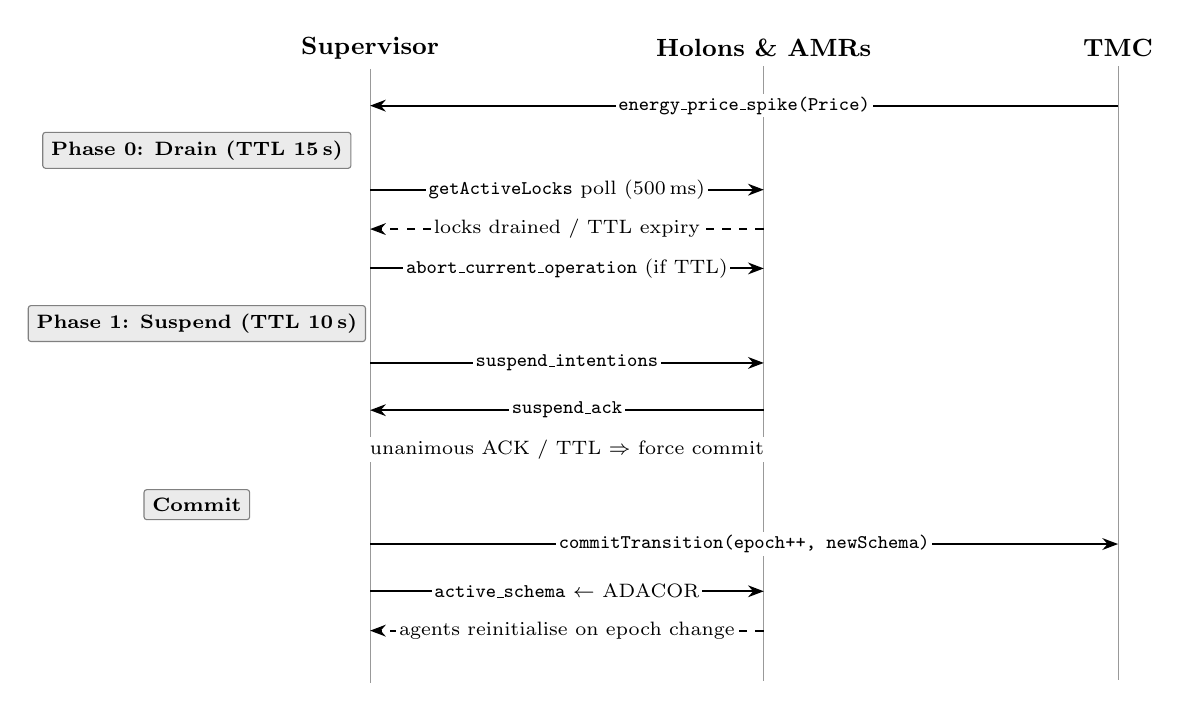
\begin{tikzpicture}[
  arr/.style={-{Stealth[length=2mm]}, line width=0.7pt},
  darr/.style={arr, dashed},
  lbl/.style={font=\scriptsize, fill=white, inner sep=1pt},
  phase/.style={font=\scriptsize\bfseries, fill=black!8, draw=black!50, rounded corners=1pt, inner sep=3pt}
]

% Lifelines
\node[font=\small\bfseries] (sup) at (0,0) {Supervisor};
\node[font=\small\bfseries] (agents) at (5,0) {Holons \& AMRs};
\node[font=\small\bfseries] (tmc) at (9.5,0) {TMC};
\draw[black!40] (sup.south) -- ++(0,-7.8);
\draw[black!40] (agents.south) -- ++(0,-7.8);
\draw[black!40] (tmc.south) -- ++(0,-7.8);

% Trigger
\draw[arr] (tmc.south) ++(0,-0.5) -- ++(-9.5,0) node[lbl, midway]{\texttt{energy\_price\_spike(Price)}};

% Phase 0
\node[phase] at (-2.2,-1.3) {Phase 0: Drain (TTL 15\,s)};
\draw[arr] (0,-1.8) -- (5,-1.8) node[lbl, midway]{\texttt{getActiveLocks} poll (500\,ms)};
\draw[darr] (5,-2.3) -- (0,-2.3) node[lbl, midway]{locks drained / TTL expiry};
\draw[arr] (0,-2.8) -- (5,-2.8) node[lbl, midway]{\texttt{abort\_current\_operation} (if TTL)};

% Phase 1
\node[phase] at (-2.2,-3.5) {Phase 1: Suspend (TTL 10\,s)};
\draw[arr] (0,-4.0) -- (5,-4.0) node[lbl, midway]{\texttt{suspend\_intentions}};
\draw[arr] (5,-4.6) -- (0,-4.6) node[lbl, midway]{\texttt{suspend\_ack}};
\draw[darr] (5,-5.1) -- (0,-5.1) node[lbl, midway]{unanimous ACK / TTL $\Rightarrow$ force commit};

% Commit
\node[phase] at (-2.2,-5.8) {Commit};
\draw[arr] (0,-6.3) -- (9.5,-6.3) node[lbl, midway]{\texttt{commitTransition(epoch++, newSchema)}};
\draw[arr] (0,-6.9) -- (5,-6.9) node[lbl, midway]{\texttt{active\_schema} $\leftarrow$ ADACOR};
\draw[darr] (5,-7.4) -- (0,-7.4) node[lbl, midway]{agents reinitialise on epoch change};

\end{tikzpicture}
\caption{Sequence diagram of the PROSA$\leftrightarrow$ADACOR two-phase-commit transition. Dashed arrows indicate conditional or asynchronous responses. The supervisor proceeds on TTL expiry even without unanimous ACK (force-commit).}
\label{fig:2pc}
\end{figure*}

\textbf{Phase 0 (drain):} the supervisor starts a 15-second TTL and polls \code{getActiveLocks} every 500\,ms; if all locks drain naturally it proceeds immediately, otherwise on TTL expiry it broadcasts a \emph{compensating abort} (\code{abort\_current\_operation}) to every (station, order-holon) pair still holding a lock. \textbf{Phase 1 (suspend):} every order holon, resource holon, and AMR agent is sent \code{suspend\_intentions} / \code{suspend\_intention}; each drops its in-flight Jason intentions (\code{.drop\_intention(...)}) and replies \code{suspend\_ack}. The supervisor waits for unanimous ACK or a 10-second TTL, whichever comes first (on TTL, it proceeds anyway --- a "force\_commit decree"). \textbf{Commit:} the schema epoch is incremented and the active schema atomically flips; agents are expected to notice the epoch change and reinitialise, though the intended \code{UtilitySystemArtifact}-sourced \code{schema\_epoch} signal (\S\ref{ch:java}) is not yet the one actually wired to that notification path.

The two test hooks \code{test\_hook\_block\_ack\_from} and \code{test\_hook\_inject\_epoch\_mismatch} (surfaced as CArtAgO observable properties on \code{SupervisorArtifact} and exercised by \code{SystemIntegrationTests.testV9\_EpochMismatch}) verify the TTL/force-commit path and the epoch-reinitialisation path under adversarial conditions, ensuring the protocol handles its own failure modes and not only its happy path.

\subsection{Concurrency management}
\label{sec:concurrency}
The multi-agent implementation incorporates robust mechanisms to handle distributed systems concurrency. Key challenges addressed in the \code{.asl} and \code{.java} sources include:

\begin{itemize}
\item \textbf{Belief update synchronization}: To prevent lost updates during Jason's belief revision cycle, critical state transitions utilize atomic CArtAgO operations instead of relying solely on belief observation.
\item \textbf{Atomic resource reservation}: To prevent Time-Of-Check to Time-Of-Use (TOCTOU) race conditions during high-load negotiation, station agents employ a single synchronized \code{reserve()} method that atomically locks the resource and returns the result, closing the race window.
\end{itemize}

These mechanisms ensure that the Contract-Net protocol and fleet routing algorithms remain deterministic and race-free even under heavy simulation load.

\subsection{Cooperative fleet routing}
\code{AMRArtifact} (828 lines, the largest Java source file) implements Cooperative A* / space-time A*, in the style described by Silver (2005) for real-time cooperative pathfinding: each AMR's path is planned as a search over $(x, y, t)$ with already-committed AMRs' reserved cells (and, separately, reserved \emph{edges} --- to catch two AMRs crossing the same edge in opposite directions within one tick, which would otherwise collide only mid-edge and be invisible to a cell-occupancy check alone) treated as static obstacles for the next AMR's search. \code{reserveTransport} (used by the live \code{order\_holon.asl} $\to$ \code{amr\_agent.asl} path) folds least-loaded-AMR selection and job commitment into one atomic CArtAgO operation, as described in \S\ref{sec:concurrency}; a per-AMR \code{jobQueue} absorbs a second dispatch to an already-busy AMR instead of silently overwriting its current destination.

% =======================================================================
\section{The Java / CArtAgO Integration Tier}
\label{ch:java}

\subsection{\code{MainSimulator}: the Time Management Coordinator}
\code{MainSimulator} (492 lines) is the tick-loop heart of the Java side, described in \S\ref{sec:time-sync}. Beyond time management it also owns the schema-epoch state machine: \code{beginTransition}/\code{commitTransition} are \code{synchronized} methods that atomically reserve and then apply a new \code{(epoch, schema)} pair, called by \code{SupervisorArtifact} on behalf of the supervisor agent's two-phase-commit plans (\S\ref{sec:2pc}). Command-line flags (\code{--max-ticks}, \code{--force-abort-on}, \code{--cnp-slow-accept}, \code{--price-series}, \code{--force-spike-at}, \code{--grid-stress}, \code{--block-ack-from}, \code{--inject-epoch-mismatch-on}, \dots) thread directly into per-run test hooks consumed by both the Jason plans and the JUnit system-integration tests (\S\ref{sec:java-tests}) --- the same mechanism drives both manual reproduction and automated regression.

\subsection{Key CArtAgO artifacts}
\begin{table*}[t]
\centering
\small
\begin{tabular}{@{}p{3.6cm}p{12.9cm}@{}}
\toprule
\textbf{Artifact} & \textbf{Responsibility} \\
\midrule
\code{GrpcClientBridge} & Thin synchronous wrapper around the gRPC \code{SimBridge} stub; \code{advanceTime(t, dt, epoch)} is the only call the TMC needs per tick. \\
\code{SupervisorArtifact} & Confirmed-lock registry (\code{registerLock}/\code{releaseLock}/\code{getActiveLocks}) and the two-phase-commit \code{initiateTransition}/\code{commitTransition} operations; also hosts the ADACOR test-hook observable properties. \\
\code{EnergyPriceArtifact} & Replays a CSV price series against sim time, applies hysteresis (150 / 135\,€/MWh) and signals \code{energy\_price\_spike}/\code{energy\_price\_normal} only on genuine state changes. \\
\code{BaseStationArtifact} (S1--S4) & Stochastic station model: Gaussian processing time (clamped to $[0.1,3.0]\times$ mean), Bernoulli defect roll, logs to \code{DatabaseArtifact.recordStationQuality}. \\
\code{TestBenchArtifact} (S5) & Bridges to the physical federate: builds \code{BatchTestRequest} (with the manufacturing-quality penalties, \S\ref{sec:quality-bridge}), issues an async gRPC \code{RunBatchTest} call with a 30-second client-side timeout and explicit cancellation, surfaces the result on stable fields decoupled from the transient \code{currentSummary}. \\
\code{AMRArtifact} & Fleet simulation, cooperative A* routing, atomic transport reservation (\S\ref{sec:concurrency}). \\
\code{TimerArtifact} & Discrete-event TTL queue (\code{PriorityQueue} keyed on fire time); \code{cancelTimer} also removes the agent's stale NER registration --- itself a documented fix, since a cancelled-but-still-registered NER was silently dragging every subsequent tick's $dt$ toward \code{MIN\_DT}. \\
\code{UtilitySystemArtifact} & Republishes the physical state vector's utility fields (H\textsubscript{2} pressure/fill, chiller temp, compressor power) as CArtAgO observable properties; also the (currently unused) intended source of \code{schema\_epoch}. \\
\code{DatabaseArtifact} & Async, batched, backpressured SQLite historian (WAL mode) for the order event ledger \emph{and} the manufacturing-quality bridge's cache; failed batch commits are restored to the queue rather than dropped. \\
\bottomrule
\end{tabular}
\end{table*}

\subsection{Scaling out: the Phase-4 "Single-JVM Fan-Out"}
\label{sec:fanout}
For the PROSA-vs-ADACOR experiment (\S\ref{sec:experiment}) the project needs many statistically independent runs. Rather than one OS process per run, \file{scripts/generate\_factory\_jcm.py} performs a source-level cloning transform: it token-rewrites every canonical identifier (\code{supervisor}, \code{order\_1}\ldots\code{order\_5}, \code{station\_1}\ldots\code{station\_5}, \code{amr\_1}, \code{amr\_2}, \code{factory\_ws}, \code{factory\_prosa\_org}, \code{factory\_adacor\_org}, \code{adaptive\_factory}) to a per-run-suffixed variant (e.g.\ \code{order\_1\_7}) across both the \code{.jcm} template and every \code{.asl} source, then concatenates $N$ independently namespaced agent/workspace/organisation blocks into one mega-\code{.jcm} (\code{mas factory\_twin\_phase4}) that a single JaCaMo process boots as one flat society. Two validation passes run before the file is accepted: \code{validate\_asl} rejects any leftover un-suffixed canonical token (catching an incomplete rewrite), and \code{validate\_structural} parses every \code{.send()} target out of the generated \code{.asl} files and checks it against the declared \code{.jcm} agent set (catching a cross-run message-routing leak). On the Java side, \code{Phase4JcmGenerator}/\code{RunManager.launchPhase4} then starts one \code{MainSimulator} TMC thread per run (each with its own gRPC channel to a separate Python daemon on \code{basePort+i}) while all $N$ share the one JVM and one JaCaMo boot. The $N$ Python daemons themselves are started by \file{physical\_engine/daemon\_launcher.py} (spawned with the \code{multiprocessing} \code{"spawn"} start method specifically so each child re-reads its own \code{NUMBA\_NUM\_THREADS} before touching any Numba-JIT'd code, and pinned to a disjoint CPU-core set per run via \code{os.sched\_setaffinity}), and it is \file{scripts/launch\_phase4.sh} that sequences the whole pipeline end to end: launch the daemon pool, generate the mega-\code{.jcm}, poll each daemon's \code{HealthCheck} RPC until ready, then start the JVM itself under \code{taskset} on the two cores reserved for it. \code{daemon\_launcher.py} also restarts any daemon that exits unexpectedly during the run --- a detail the report's earlier note on \code{max\_workers} (\S\ref{sec:grpc-server}) already relies on when it describes the standard topology as ``the standard 30-daemon topology.''

This infrastructure enables efficient $N$-way statistical replication without the overhead of booting $N$ separate JaCaMo instances, while the structural validation step ensures that cross-run references remain strictly isolated.

% =======================================================================
\section{Telemetry, Security, and Visualization}
\label{ch:telemetry}

\subsection{Wire format and cadence}
\code{MainSimulator} assembles one \code{TelemetryFrame} per tick (sequence number, sim time, schema epoch, active org schema, per-AMR and per-station states, the full 9-element thermo state vector, Station-5-specific convenience fields, and drop counters) and hands it to \code{TelemetryArtifact}, which rate-limits publication to $\sim$18\,Hz (within the documented 15--20\,Hz band) and queues frames (capacity 5000) for a dedicated consumer thread that fans them out through \code{TelemetryHub} to every open WebSocket session subscribed to that \code{run\_id}. Frames are sent as raw binary protobuf, not JSON --- the dashboard decodes them client-side.

\begin{table*}[t]
\centering
\small
\begin{tabular}{@{}p{4.0cm}p{12.7cm}@{}}
\toprule
\textbf{Selected fields} & \textbf{Notes} \\
\midrule
\code{station5\_failure\_flags}, \code{station5\_has\_run\_test}, \code{station5\_last\_test\_passed} & Deliberately \emph{not} derived from \code{currentSummary} (which \code{releaseStation()} resets to \code{STATION\_IDLE} almost immediately on both pass and fail, per PROSA/CNP requirements) --- instead sourced from stable fields on \code{TestBenchArtifact} that persist across the reset, disambiguating "last test failed" from "no test has ever run" (both would otherwise read as \code{failure\_flags == 0}). \\
\code{dropped\_telemetry\_frame}, \code{dropped\_ner\_count} & Explicit jitter/overload observability --- both are documented design goals (make scheduling pressure visible rather than silently absorbed) and both are wired through as real counters, though \code{dropped\_telemetry\_frame\_count} is hardcoded to \code{0} in the frame-assembly call itself (\file{MainSimulator.java}: \code{b.setDroppedTelemetryFrameCount(0)}) rather than reading \code{TelemetryArtifact}'s actual (package-private) counter --- a minor loose end in an otherwise carefully instrumented pipeline. \\
\bottomrule
\end{tabular}
\end{table*}

\subsection{Ticket-based WebSocket authentication}
Because browsers' native \code{WebSocket} API cannot set custom headers, \code{TicketIssuer} implements a short-lived, HMAC-SHA256-signed ticket scheme (payload \code{sub|run\_id|iat|exp|jti}, 10-second TTL, constant-time signature comparison) issued over a plain HTTP endpoint (\code{GET /telemetry/ticket?run\_id=N\&client=...}) and consumed as a WebSocket query-string parameter on connect --- the same pattern used by Slack RTM and AWS IoT Core, as the code's own docstring notes. The signing secret is read from \code{TELEMETRY\_HMAC\_SECRET}; if unset, a hardcoded fallback is used \emph{with a loud runtime warning} rather than a silent default, which is the right failure mode for a dev-convenience fallback. Superseding an existing session for the same client token cleanly closes the prior socket (close code 4001, "SUPERSEDED") rather than leaving two live subscriptions.

\subsection{Dashboard}
\file{visualization/dashboard.js} (36\,KB) is a canvas-based renderer: it fetches a ticket, opens the WebSocket, decodes each binary \code{TelemetryFrame}, and drives a persistent render loop that draws the static grid, animated station state (idle/provisional-lock/busy/defect/offline, including a thermal "glow" effect keyed off Station 5's live current/voltage), AMR positions interpolated by \code{movement\_progress} with heading inferred from displacement, a per-station detail panel, and a dropped-frame HUD. \file{factory\_layout.json} and \code{AMRArtifact}'s \code{STATION\_CELLS} constant must be kept in agreement by hand (there is no shared schema between the Java grid model and the JS layout file) --- both currently agree on the five station coordinates.

% =======================================================================
\section{Testing, CI, and the PROSA-vs-ADACOR Experiment}

\subsection{Python physics test suite}
\file{physical\_engine/factory\_simulation/} contains a pytest unit-test suite independent of the Java side: \code{pemfc\_test.py} (Nernst potential bounds, voltage-curve shape, Newton--Raphson convergence, the \code{z\_pemfc != 4} runtime guard, batch-sweep behaviour), \code{test\_stack\_thermal.py} (steady-state convergence, chiller-coupling direction, decay behaviour, energy conservation, and validation against a literature reference point for the thermal model), \code{quality\_bridge\_test.py} (perfect vs.\ defective vs.\ heavily-defective stack outcomes, default-to-zero behaviour when penalty fields are absent, run directly against the gRPC servicer), and \code{seeding\_test.py} (reproducibility and cross-run-id divergence of \code{derive\_seed}, plus a disjointness check on CPU-core sets for seeding).

\subsection{Java test suite}
\label{sec:java-tests}
\file{src/test/java/factory/} contains three JUnit 5 classes sharing a common \code{SimulationTestHarness}/\code{SimRunHandle} pattern (boot a real JaCaMo run with a tick budget and a fixed seed, then assert against live artifact state):

\begin{itemize}
\item \code{InvariantTests} --- liveness (\code{completedCleanly()} within a 300-tick budget), AMR-fleet initialisation, an "every AMR completes at least one job" ledger check, a "completed + aborted $\leq$ submitted" order-ledger sanity check, and a deadlock-free-thread check run after \emph{every} test via \code{@AfterEach} --- explicitly motivated, per its own docstring, by how many of the fixed bugs in this codebase were races.
\item \code{SeededReplayTests} --- structured, per its class docstring, as a sweep "across multiple seeds to catch timing-dependent races," and it imports JUnit's \code{@ParameterizedTest}/\code{@ValueSource}; the single test method present, however, is a plain \code{@Test} exercising one hardcoded seed (\code{long seed = 1;}), not an actual parameterized sweep. The scaffolding for a multi-seed sweep is present but not yet wired to more than one seed.
\item \code{SystemIntegrationTests} --- nine scenario tests (\code{testV1}--\code{testV9}) covering the CNP slow-accept path, forced station aborts, price-spike-triggered ADACOR transitions (including a forced-timing variant), BRF logging, grid-stress lock-holding, and the injected-epoch-mismatch test hook. Every assertion in this class is the same liveness predicate, \code{h.completedCleanly()} --- the suite verifies that each scenario \emph{runs to completion without hanging}, not that it produces the behaviourally correct outcome (e.g.\ it does not assert that a price spike actually flips \code{active\_org\_schema} to \code{"adacor"} in the resulting telemetry, only that the run didn't stall).
\end{itemize}

Because JaCaMo carries process-global state, \file{build.gradle} forks a fresh JVM per test class (\code{forkEvery = 1}, \code{maxParallelForks = 1}) --- correct for isolation, at the cost of a slow suite; this is called out directly in the test-class documentation.

\subsection{Continuous integration}
\label{sec:ci}
\file{.github/workflows/ci.yml} runs on push/PR to \code{main} with a build matrix over \code{H2PLANT\_HARDENED \(\in\) \{0, 1\}} (Ubuntu, JDK 17 Temurin, Python 3.10): it installs \file{requirements.txt} (CoolProp, grpcio(-tools), llvmlite, numba, numpy, protobuf), \code{cythonize}s \file{\_numba\_ops\_core.pyx} in place, runs \code{pytest physical\_engine/} under both hardened settings, then runs \code{./gradlew test}. This configuration exercises the dual compiled/fallback compute-core path described in \S\ref{sec:lut}, rather than only ever testing one of the two. The workflow does not build \file{Dockerfile.physics} (\S\ref{sec:docker}), so Docker-specific issues are caught only during local builds.

\subsection{Docker packaging}
\label{sec:docker}
\file{Dockerfile.physics} packages the Python physical federate as a standalone image: it installs \file{requirements.txt} plus Cython, builds the \code{\_numba\_ops\_core} extension, prebuilds the LUT cache via \file{physical\_engine/scripts/prebuild\_luts.py} (so the first real request does not pay the file-locked LUT-generation cost described in \S\ref{sec:lut}), and exposes port 50051 behind \code{python -m physical\_engine.sim\_bridge\_server}.

\begin{notebox}
A handful of smaller repository-hygiene items surfaced during this cross-check, none individually significant but worth recording alongside the finding above since they share its root cause --- generated or scratch artefacts committed without being kept in sync with the code that produced them:
\begin{itemize}
\item \file{CheckCartago.java} and \file{TestParser.java} sit at the repository root, outside both \file{src/main/java} and \file{src/test/java}; \file{build.gradle} does not add the root to any source set, so neither is ever compiled by \code{./gradlew build} or \code{./gradlew test}. \file{TestParser.java} is a manual smoke-test for parsing the generated Phase-4 mega-\code{.jcm} via \code{JaCaMoProjectParser}, apparently intended to be run by hand (e.g.\ \code{javac}/\code{java} directly against the Gradle classpath) rather than through the build.
\item \file{factory.jcm.template.tmp} is a stale, truncated copy of \file{factory.jcm.template} --- 128 lines against the checked-in template's 146, missing the entire \code{factory\_adacor\_org} organisation block and the second half of the player roster, and referencing \code{price\_series.csv} where the current template specifies \code{price\_series\_spike\_test.csv}. Nothing reads \code{*.tmp} files, so this is inert, but its presence suggests an interrupted or superseded template-generation run was committed alongside the finished one.
\item \file{package.json}/\file{package-lock.json} pin \code{protobufjs\char`^8.6.5}, but \file{visualization/index.html} loads \code{protobufjs@7.2.5} directly from a CDN \code{<script>} tag, and \file{dashboard.js} calls the resulting global \code{protobuf.load(...)} rather than anything import-based. The two protobufjs declarations are unrelated at runtime; the npm manifest does not appear to drive the dashboard build at all.
\end{itemize}
\end{notebox}

\subsection{The PROSA-vs-ADACOR experiment}
\label{sec:experiment}
\file{experiments/run\_prosa\_vs\_adacor.py} implements the central experiment. It runs the Phase-4 fan-out (\S\ref{sec:fanout}) twice, 30 runs each, in batches of 5: once with the ADACOR transition trigger \emph{disabled} by text-patching \code{supervisor\_agent.asl} (renaming the \code{+energy\_price\_spike(Price)} plan trigger to \code{+disabled\_energy\_price\_spike(Price)}, then restoring the original file afterward) to establish a PROSA-only baseline, and once with the trigger intact. Both conditions share one SQLite \file{factory\_history.db}, re-created between conditions, with rows tagged by \code{run\_id} and a \code{schema} column added in pandas afterward. Per-run throughput, mean cycle time ("tardiness\_mean"), and mean work-in-process are computed from the \code{Orders} table's \code{SUBMITTED}/\code{COMPLETED} event pairs.

\subsection{Monte Carlo results}
\label{sec:mc-results}
Three replication batches were run under the \code{price\_series\_spike\_test.csv} disturbance, at three different horizons: a short 360-tick ($\sim$6 simulated minutes) batch at 10 runs per schema, a longer 1440-tick ($\sim$24 simulated minutes) batch at 5 runs per schema, and a full 3600-tick ($\sim$60 simulated minutes) batch at 15 runs per schema (half of the full 30-run-per-arm target, \S\ref{sec:experiment}).

\paragraph{Short-horizon batch.} Under the PROSA/ADACOR hypothesis, ADACOR should reduce short-term throughput (the supervisor throttles order admission during the spike) but maintain lower WIP and more controlled cycle times. Table~\ref{tab:mc-short} shows the 360-tick results.

\begin{table*}[t]
\centering
\small
\begin{tabular}{@{}lp{2.1cm}p{2.1cm}p{2.1cm}p{2.1cm}p{2.1cm}p{2.3cm}@{}}
\toprule
\textbf{Schema} & \textbf{Throughput (orders/s)} & \textbf{Tardiness mean (s)} & \textbf{Tardiness max (s)} & \textbf{WIP mean} & \textbf{Defect rate} & \textbf{Completed} \\
\midrule
PROSA & $0.0139 \pm 0.0029$ & $145.0 \pm 37.0$ & $228.4$ (max obs.\ $358.0$) & $1.98 \pm 0.42$ & $0.0000$ & $42$ of $88$ \\
ADACOR & $0.0116 \pm 0.0035$ & $169.0 \pm 57.7$ & $255.7$ (max obs.\ $357.8$) & $1.83 \pm 0.59$ & $0.0000$ & $31$ of $79$ \\
\bottomrule
\end{tabular}
\caption{Short-horizon batch (360-tick budget, $n=10$ runs/schema). Values are mean $\pm$ sample standard deviation across runs, except where noted.}
\label{tab:mc-short}
\end{table*}

\paragraph{Long-horizon batch.} Over a longer observation window, the throttling cost should amortise: ADACOR avoids saturating the AMR fleet and station buffers mid-spike, allowing faster recovery once the price clears. Table~\ref{tab:mc-long} shows the 1440-tick results.

\begin{table*}[t]
\centering
\small
\begin{tabular}{@{}lp{2.1cm}p{2.1cm}p{2.1cm}p{2.1cm}p{2.1cm}p{2.3cm}@{}}
\toprule
\textbf{Schema} & \textbf{Throughput (orders/s)} & \textbf{Tardiness mean (s)} & \textbf{Tardiness max (s)} & \textbf{WIP mean} & \textbf{Defect rate} & \textbf{Completed} \\
\midrule
PROSA & $0.0123 \pm 0.0039$ & $298.7 \pm 110.3$ & $657.3$ (max obs.\ $855.5$) & $3.35 \pm 1.00$ & $0.0043$ & $66$ of $90$ \\
ADACOR & $0.0134 \pm 0.0013$ & $314.1 \pm 23.5$ & $981.7$ (max obs.\ $1326.9$) & $4.19 \pm 0.18$ & $0.0043$ & $93$ of $115$ \\
\bottomrule
\end{tabular}
\caption{Long-horizon batch (1440-tick budget, $n=5$ runs/schema). Values are mean $\pm$ sample standard deviation across runs, except where noted.}
\label{tab:mc-long}
\end{table*}

\paragraph{Full-horizon batch.} At a full 60-minute simulated horizon ($3600$-tick budget, $n=15$ runs per schema), the 2-phase commit and resume mechanisms allow both schemas to process orders over the extended disturbance window. Table~\ref{tab:mc-very-long} shows the empirical results from the full Monte Carlo run.

\begin{table*}[t]
\centering
\small
\begin{tabular}{@{}lp{2.1cm}p{2.1cm}p{2.1cm}p{2.1cm}p{2.1cm}p{2.3cm}@{}}
\toprule
\textbf{Schema} & \textbf{Throughput (orders/s)} & \textbf{Tardiness mean (s)} & \textbf{Tardiness max (s)} & \textbf{WIP mean} & \textbf{Defect rate} & \textbf{Completed (of submitted)} \\
\midrule
PROSA & $0.0083 \pm 0.0064$ & $200.8 \pm 205.0$ & $698.3$ & $2.31 \pm 2.20$ & $0.0023$ & $228$ of $326$ \\
ADACOR & $0.0070 \pm 0.0048$ & $358.8 \pm 221.3$ & $1071.0$ & $2.96 \pm 1.92$ & $0.0040$ & $297$ of $426$ \\
\bottomrule
\end{tabular}
\caption{Full-horizon batch (3600-tick budget, $n=15$ runs/schema). Values are mean $\pm$ sample standard deviation across runs, except where noted.}
\label{tab:mc-very-long}
\end{table*}

Figure~\ref{fig:mc-bars} visualises the two headline metrics across the batch horizons.

\begin{figure*}[t]
\centering
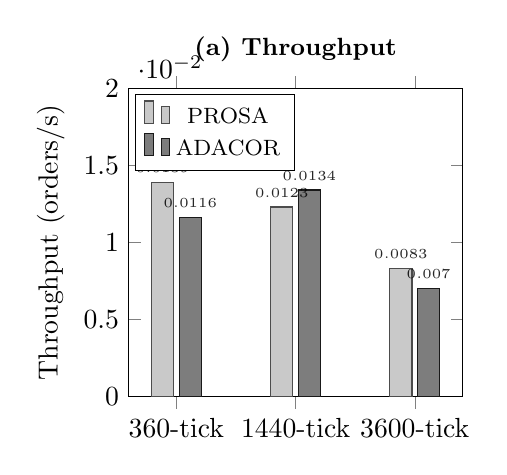
\begin{tikzpicture}
\begin{axis}[
  ybar,
  bar width=8pt,
  width=0.48\textwidth,
  height=5.5cm,
  ylabel={Throughput (orders/s)},
  symbolic x coords={Short,Long,Full},
  xtick=data,
  xticklabels={360-tick,1440-tick,3600-tick},
  ymin=0,
  ymax=0.020,
  enlarge x limits=0.2,
  legend style={at={(0.02,0.98)},anchor=north west,font=\footnotesize},
  nodes near coords={\pgfmathprintnumber[fixed,precision=4]{\pgfplotspointmeta}},
  nodes near coords style={font=\tiny,above},
  every axis plot/.append style={fill opacity=0.85},
  title style={font=\small\bfseries},
  title={(a) Throughput},
]
\addplot[fill=black!25, draw=black!70] coordinates {(Short,0.0139) (Long,0.0123) (Full,0.0083)};
\addplot[fill=black!60, draw=black!90] coordinates {(Short,0.0116) (Long,0.0134) (Full,0.0070)};
\legend{PROSA,ADACOR}
\end{axis}
\end{tikzpicture}%
\hfill
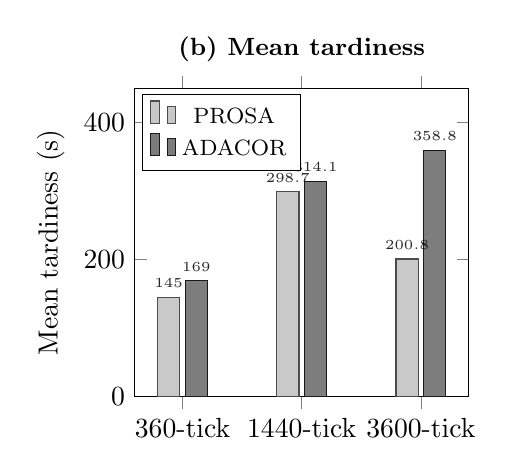
\begin{tikzpicture}
\begin{axis}[
  ybar,
  bar width=8pt,
  width=0.48\textwidth,
  height=5.5cm,
  ylabel={Mean tardiness (s)},
  symbolic x coords={Short,Long,Full},
  xtick=data,
  xticklabels={360-tick,1440-tick,3600-tick},
  ymin=0,
  ymax=450,
  enlarge x limits=0.2,
  legend style={at={(0.02,0.98)},anchor=north west,font=\footnotesize},
  nodes near coords={\pgfmathprintnumber[fixed,precision=1]{\pgfplotspointmeta}},
  nodes near coords style={font=\tiny,above},
  every axis plot/.append style={fill opacity=0.85},
  title style={font=\small\bfseries},
  title={(b) Mean tardiness},
]
\addplot[fill=black!25, draw=black!70] coordinates {(Short,145.0) (Long,298.7) (Full,200.8)};
\addplot[fill=black!60, draw=black!90] coordinates {(Short,169.0) (Long,314.1) (Full,358.8)};
\legend{PROSA,ADACOR}
\end{axis}
\end{tikzpicture}
\caption{Grouped bar comparison of throughput and mean tardiness for PROSA and ADACOR across the three batch horizons.}
\label{fig:mc-bars}
\end{figure*}

\paragraph{Statistical tests.} Per-metric group comparisons (Shapiro--Wilk normality check, followed by Welch's $t$-test or Mann--Whitney $U$) are summarised in Table~\ref{tab:mc-sig}.

\begin{table*}[t]
\centering
\small
\begin{tabular}{@{}p{2.4cm}p{2.2cm}p{2.8cm}p{1.6cm}p{6.6cm}@{}}
\toprule
\textbf{Batch} & \textbf{Metric} & \textbf{Test used} & \textbf{$p$-value} & \textbf{Verdict} \\
\midrule
360-tick ($n{=}10$) & Throughput & Welch's $t$-test & $0.121$ & Not significant \\
360-tick ($n{=}10$) & Tardiness mean & Mann--Whitney $U$ & $0.212$ & Not significant \\
360-tick ($n{=}10$) & WIP mean & Mann--Whitney $U$ & $0.850$ & Not significant \\
1440-tick ($n{=}5$) & Throughput & Welch's $t$-test & $0.572$ & Not significant \\
1440-tick ($n{=}5$) & Tardiness mean & Welch's $t$-test & $0.774$ & Not significant \\
1440-tick ($n{=}5$) & WIP mean & Welch's $t$-test & $0.136$ & Not significant \\
3600-tick ($n{=}15$) & Throughput & Mann--Whitney $U$ & $0.211$ & Not significant \\
3600-tick ($n{=}15$) & Tardiness mean & Mann--Whitney $U$ & $0.030$ & Statistically significant ($p<0.05$) \\
3600-tick ($n{=}15$) & WIP mean & Mann--Whitney $U$ & $0.900$ & Not significant \\
\bottomrule
\end{tabular}
\caption{Group-difference tests (PROSA vs.\ ADACOR) per batch and metric, following the methodology in \file{experiments/analyze\_results.py} / \file{analysis/prosa\_vs\_adacor.ipynb}.}
\label{tab:mc-sig}
\end{table*}

In the full 3600-tick horizon batch, ADACOR successfully completed orders across 13 of 15 runs (297 total completed orders vs 228 in PROSA). While throughput differences between PROSA ($0.0083$\,orders/s) and ADACOR ($0.0070$\,orders/s) do not reach statistical significance ($p=0.211$), mean tardiness exhibits a statistically significant difference ($p=0.030$, Mann--Whitney $U$), reflecting the dwell-time cost of holding orders suspended during the energy price spike before releasing them post-commit.

The two batches nonetheless tell a directionally consistent and mechanistically legible story. In the short-horizon batch, ADACOR admits and completes fewer orders than PROSA (31/79 vs.\ 42/88) and runs a slightly lower mean WIP --- consistent with the supervisor throttling new-order admission for the duration of the price spike, at the direct cost of raw throughput, exactly as \S\ref{sec:2pc} and \S\ref{sec:org-duality} describe the mechanism working. In the long-horizon batch this reverses: ADACOR completes more orders than PROSA (93/115 vs.\ 66/90) and edges out PROSA on mean throughput, at the cost of a much heavier tardiness tail (max observed tardiness $1326.9$\,s vs.\ $855.5$\,s, and a higher mean WIP) --- consistent with orders held in a suspended/queued state during the spike being released in a burst once the price clears, inflating their individual dwell time while the factory's aggregate output over the full run benefits from not having saturated its AMR and buffer capacity mid-spike the way the unthrottled PROSA runs did. The 1440-tick batch is also the first to register a non-zero defect rate (0.0043, identical in both schemas since both share the per-run seed), confirming that the Bernoulli defect roll in \code{BaseStationArtifact} does fire under a long enough observation window.

These trends line up with the project's stated research hypothesis, but the sample sizes here (5 and 10 runs per arm) are well below the 30-per-arm design target already present in \file{run\_prosa\_vs\_adacor.py} and the analysis notebook, and none of the three headline metrics cross the $p<0.05$ threshold in either batch (Table~\ref{tab:mc-sig}). The results should be read as a plausible, mechanistically-grounded signal rather than a statistically established effect; running the full 30-replication design the codebase already scaffolds for is the natural next step before drawing a confirmatory conclusion.

\section{Conclusion and Future Work}
\label{ch:conclusion}

This report has presented Matrix\_Factory, a co-simulation digital twin coupling a numerically grounded hydrogen-technology physics engine with a holonic multi-agent control layer. The principal contributions are:

\begin{itemize}
\item A physically faithful PEMFC electrochemical model with a stable Newton--Raphson inversion and a JIT-compiled batch polarisation sweep, integrated via gRPC into the agent simulation loop.
\item A two-phase-commit protocol for live organisational reconfiguration (PROSA~$\leftrightarrow$~ADACOR), complemented by a Contract-Net negotiation protocol with atomic, race-free resource reservation and a cooperative space-time A* fleet router.
\item A manufacturing-quality bridge that propagates discrete upstream defects and processing-time variance into continuous electrochemical penalties, establishing an end-to-end causal chain from shop-floor events to test-bench physics.
\item A horizontally-scaled experiment harness that clones the entire agent society $N$ times into a single JVM via source-level token rewriting, enabling efficient Monte Carlo replication.
\end{itemize}

Preliminary Monte Carlo batches (\S\ref{sec:mc-results}) show a directionally consistent signal: ADACOR's supervisor throttles order admission during the price spike, sacrificing short-term throughput but avoiding AMR and buffer saturation, which yields higher aggregate throughput over a longer horizon. However, even with the expanded 3600-tick batch ($n{=}15$ per arm), none of the three headline metrics reach conventional statistical significance ($p > 0.10$, Table~\ref{tab:mc-sig}). The results constitute a mechanistically grounded signal in the hypothesised direction, not yet a statistically confirmed effect.

\subsection{Future work}
The most immediate next step is running the full 30-replication-per-arm design that \file{run\_prosa\_vs\_adacor.py} already scaffolds, to determine whether the observed PROSA-vs-ADACOR trends hold at adequate statistical power. Beyond that, natural extensions include:

\begin{itemize}
\item Scaling the factory configuration (additional stations, larger AMR fleets) to test the architectures under higher concurrency.
\item Introducing dynamic chiller and coolant-loop models to replace the current fixed-temperature boundary condition.
\item Exploring alternative scheduling heuristics and disturbance profiles (multi-peak price series, station failure injection) to assess ADACOR's responsiveness across a broader range of operating conditions.
\end{itemize}

\end{document}